\documentclass[tikz]{standalone}

\usepackage{tikz}
\usetikzlibrary{decorations}
\usetikzlibrary{decorations.pathreplacing, intersections}
\usepackage{pgfplots}
\usetikzlibrary{calc,positioning}
\pgfplotsset{compat=newest, scale only axis, width = 10cm}

% Create fake \onslide and other commands for standalone picture
\usepackage{xparse}
\NewDocumentCommand{\onslide}{s t+ d<>}{}
\NewDocumentCommand{\only}{d<>}{}
\NewDocumentCommand{\uncover}{d<>}{}
\NewDocumentCommand{\visible}{d<>}{}
\NewDocumentCommand{\invisible}{d<>}{}

\begin{document}

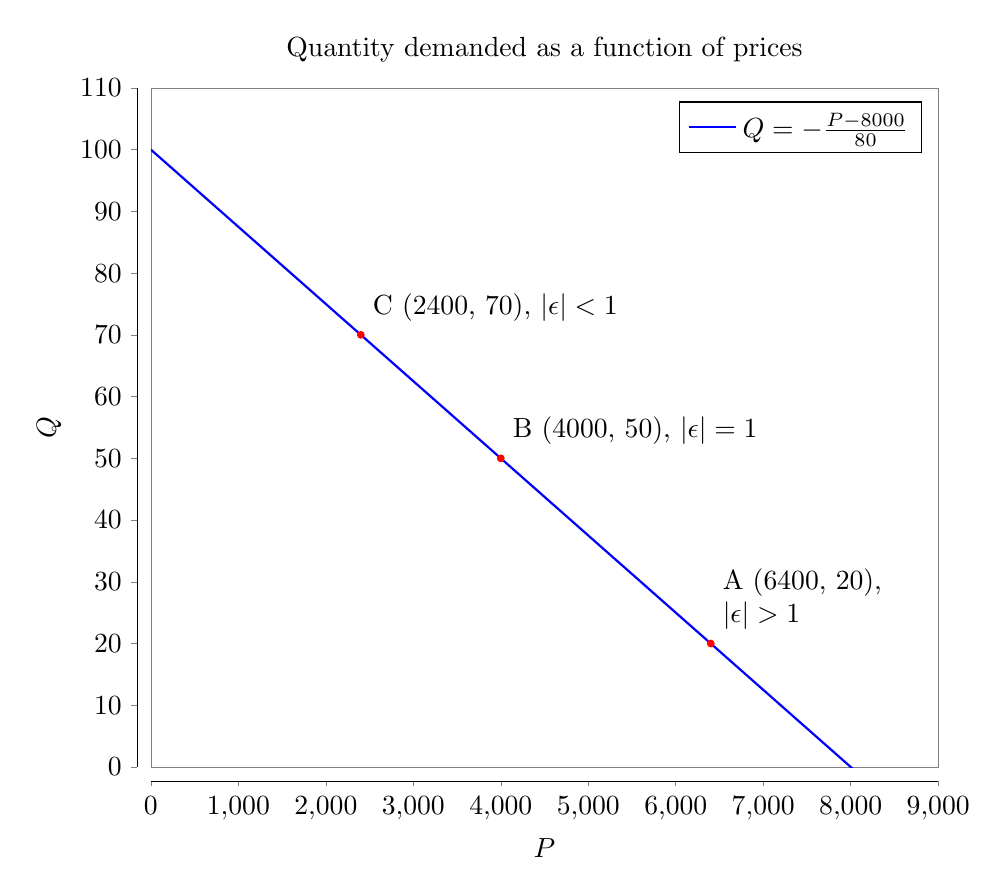
\begin{tikzpicture}
\begin{axis}[
    xmin = 0,
    ymax = 110,
    ymin = 0,
    xmax = 9000,
    xlabel = {$P$},
    ylabel = {$Q$},
    sciclean/.style={axis lines=left,
        axis x line shift=0.5em,
        axis y line shift=0.5em,
        axis line style={-,very thin},
        axis background/.style={draw,ultra thin,gray},
        tick align=outside,
        xtick distance=1000,
        ytick distance=10,
        major tick length=2pt},
    title = {Quantity demanded as a function of prices},
    sciclean]
\addplot[thick, color = blue, domain = 0:9000] {-(x - 8000) / 80};
\addlegendentry{$ Q =  -\frac{P - 8000}{80}$}
\node[label = {[align=left] 60:A (6400, 20), \\ $ |\epsilon| > 1 $}, fill=red,circle,inner sep=1pt] at (axis cs:6400, 20) {} ;
\node[label = {60:B (4000, 50), $ |\epsilon| = 1$}, fill=red,circle,inner sep=1pt] at (axis cs:4000, 50) {} ;
\node[label = {60:C (2400, 70), $ |\epsilon| < 1 $}, fill=red,circle,inner sep=1pt] at (axis cs:2400, 70) {} ;
\end{axis}
\end{tikzpicture}
\end{document}
